\documentclass{exam}
\usepackage[utf8]{inputenc}
\usepackage{lmodern}
\usepackage{microtype}

% \usepackage[parfill]{parskip}
\usepackage[dvipsnames]{xcolor}
\usepackage{amsmath}
\usepackage{amsfonts}
\usepackage{amsthm}
\usepackage{siunitx}
\DeclareSIUnit\year{yr}
\DeclareSIUnit\foot{ft}
\DeclareSIUnit\litre{\liter}

\usepackage{skull}

\usepackage{pgfplots}
\usepgfplotslibrary{polar}
\pgfplotsset{compat=1.11}
\usepgfplotslibrary{statistics}
\usepackage{graphicx}
\usepackage{sidecap}
\sidecaptionvpos{figure}{c}
\usepackage{float}
\usepackage{gensymb}
\usepackage{tkz-euclide}
\usetkzobj{all}
\usepackage{commath}
\usepackage{hyperref}
\usepackage{enumitem}
\usepackage{wasysym}
\usepackage{multicol}
\usepackage{mathtools}
\usepackage{tcolorbox}
\usepackage{tabularx}
\usepackage[version=4]{mhchem}
\usepackage{changepage}
\usepackage{listings}
\lstset{basicstyle=\ttfamily\linespread{0.8}\small}

\renewcommand*{\thefootnote}{\fnsymbol{footnote}}

\newtheorem*{thm}{Theorem}
\newtheorem*{iden}{Identity}
\newtheorem*{lemma}{Lemma}
\newtheorem{obs}{Observation}
\theoremstyle{definition}
\newtheorem*{defn}{Definition}
\newtheorem*{ex}{Example}
\newtheorem{con}{Construction}
\newtheorem*{alg}{Algorithm}

\newtheoremstyle{break}
  {\topsep}{\topsep}%
  {\itshape}{}%
  {\bfseries}{}%
  {\newline}{}%
\theoremstyle{break}
\newtheorem*{bthm}{Theorem}

% russian integral
\usepackage{scalerel}
\DeclareMathOperator*{\rint}{\scalerel*{\rotatebox{17}{$\!\int\!$}}{\int}}

% \DeclareMathOperator*{\rint}{\int}

\pgfplotsset{vasymptote/.style={
    before end axis/.append code={
        \draw[densely dashed] ({rel axis cs:0,0} -| {axis cs:#1,0})
        -- ({rel axis cs:0,1} -| {axis cs:#1,0});
    }
}}

% \pointsinrightmargin
\boxedpoints
\pointname{}

\newcommand{\questioA}{\question[\texttt{\textbf{\color{Cerulean} A}}]}
\newcommand{\questioM}{\question[\texttt{\textbf{\color{PineGreen} M}}]}
\newcommand{\questioE}{\question[\texttt{\textbf{\color{WildStrawberry} E}}]}
\newcommand{\questioS}{\question[\texttt{\textbf{\color{Goldenrod} S}}]}
\newcommand{\questioO}{\question[\texttt{\textbf{\color{BurntOrange} O}}]}

\newcommand{\parA}{\part[\texttt{\textbf{\color{Cerulean} A}}]}
\newcommand{\parM}{\part[\texttt{\textbf{\color{PineGreen} M}}]}
\newcommand{\parE}{\part[\texttt{\textbf{\color{WildStrawberry} E}}]}
\newcommand{\parS}{\part[\texttt{\textbf{\color{Goldenrod} S}}]}
\newcommand{\parO}{\part[\texttt{\textbf{\color{BurntOrange} O}}]}

\newcommand{\subparA}{\subpart[\texttt{\textbf{\color{Cerulean} A}}]}
\newcommand{\subparM}{\subpart[\texttt{\textbf{\color{PineGreen} M}}]}
\newcommand{\subparE}{\subpart[\texttt{\textbf{\color{WildStrawberry} E}}]}
\newcommand{\subparS}{\subpart[\texttt{\textbf{\color{Goldenrod} S}}]}
\newcommand{\subparO}{\subpart[\texttt{\textbf{\color{BurntOrange} O}}]}

\newcommand{\mainHeader}[2]{\section*{NCEA Level 2 Mathematics\\#1. #2}}
\newcommand{\mainHeaderHw}[2]{\section*{NCEA Level 2 Mathematics (Homework)\\#1. #2}}
\newcommand{\seealso}[1]{\begin{center}\emph{See also #1.}\end{center}}
\newcommand{\drills}[1]{\begin{center}\emph{Drill problems: #1.}\end{center}}
\newcommand{\basedon}[1]{\begin{center}\emph{Notes largely based on #1.}\end{center}}


\begin{document}

\mainHeader{8}{The Quadratic Formula}
\subsection*{Solving Quadratics}
Recall that a quadratic equation is one of the form $ y = ax^2 + bx + c $ (where $ a \neq 0 $). A couple of weeks ago, we saw that we
can always rearrange such an equation into vertex form; we do this by trying to rewrite it as a square plus a constant. This process
is known as \emph{completing the square}.

Our goal is to end up with something that looks like
\begin{displaymath}
  y = \alpha(x + \beta)^2 + \gamma
\end{displaymath}
where $ (-\beta,\gamma) $ are the coordinates of the vertex of the parabola and $ \alpha $ (as we have seen) is the `scaling factor'
that gives us the shape. If $ \alpha $ is negative then the parabola opens downwards, and if $ \alpha $ is positive then the parabola
opens upwards.

If we expand the parabola equation, we obtain
\begin{align*}
  y &= \alpha (x^2 + \beta x + \beta^2) + \gamma\\
    &= \alpha x^2 + 2\alpha \beta x + \alpha \beta^2 + \gamma.
\end{align*}
By comparing coefficients, we see that:
\begin{align*}
  a &= \alpha\\
  b &= 2\alpha \beta = 2a\beta\\
  c &= \alpha\beta^2 + \gamma = a\beta^2 + \gamma.
\end{align*}
Clearly, then, we have $ \beta = b/2a $. Substituting this into the third equation, we have $ c = a(b/2a)^2+ \gamma $
and so $ \gamma = c - \frac{b^2}{4a} $.

Reasoning thusly, we see that
\begin{displaymath}
  y = ax^2 + bx + c = \alpha(x + \beta)^2 + \gamma = a\left(x + \frac{b}{2a}\right)^2 + c - \frac{b^2}{4a},
\end{displaymath}
which is what I asked you to prove in the homework when we looked at parabolae.

\begin{ex}
  Suppose we are given a rectangular plot of land and are told that the area of the land is \SI{32}{\kilo\metre\squared} and that
  one side of the land is \SI{8}{\kilo\metre} longer than the other. In order to find the dimensions of the land, we have a quadratic
  equation which we can simplify:
  \begin{displaymath}
    x(x + 8) = 32 \implies x^2 + 8x - 32 = 0.
  \end{displaymath}
  Completing the square, we have that
  \begin{displaymath}
    0 = (x + 4)^2 - 16 + (-32) = (x + 4)^2 - 48
  \end{displaymath}
  and so $ x = \sqrt{48} - 4 \approx \SI{2.9}{\kilo\metre} $.
\end{ex}

This example suggests that we can write down a formula for the value of $ x $ in any quadratic equation $ 0 = ax^2 + bx + c $
by rewriting that equation in vertex form and solving for $ x $:
\begin{gather*}
  0 = ax^2 + bx + c = a\left(x + \frac{b}{2a}\right)^2 + c - \frac{b^2}{4a}\\
  \frac{b^2}{4a} - c = a\left(x + \frac{b}{2a}\right)^2\\
  \pm\sqrt{\frac{b^2}{4a^2} - \frac{c}{a}} = x + \frac{b}{2a}\\
  - \frac{b}{2a} \pm\sqrt{\frac{b^2}{4a^2} - \frac{4ac}{4a^2}} = x\\
  \frac{-b \pm \sqrt{b^2 - 4ac}}{2a} = x.
\end{gather*}

We have therefore proved the following
\begin{thm}[Quadratic formula]
  If $ ax^2 + bx + c = 0 $, then there are at most two distinct values for $ x $. These values are given by
  \begin{displaymath}
    x = \frac{-b \pm \sqrt{b^2 - 4ac}}{2a}
  \end{displaymath}
  when they exist.
\end{thm}

These values are called the \emph{solutions}, the \emph{roots}, or the \emph{zeroes} of the equation.

\begin{ex}
  The width of a canal at ground level is \SI{16}{\metre}. The sides of the canal can  be modelled by a quadratic expression
  that would give a maximum depth of \SI{16}{\metre}. However, the base of the canal is flat and has a width of \SI{12}{\metre}.
  What is the depth of the canal?

  \textit{Solution.} Model the canal with $ y = a(x + 8)(x - 8) $. This parabola passes through $ (0, -16) $, so we have $ -16 = a(+8)(-8) $
  and hence $ a = \frac{16}{64} = \frac{1}{4} $; so $ y = \frac{1}{4}(x + 8)(x - 8) $.

  The width of the parabola is $ 12 $ at the $ y$--value corresponding to the $ x$--values $ \pm 6 $; at $ x = \pm 6 $, $ y = -7 $
  and so the depth of the canal is \SI{7}{\metre}.
\end{ex}

\clearpage
\subsection*{Forms of a Quadratic}
We have seen that there are three complementary ways of viewing the equation $ y = ax^2 + bx + c $, each of which
exhibits one particular characteristic of the function:
\begin{center}
  \begin{tabular}{l|l|l}
    \textbf{Form} & \textbf{Exhibits} & \textbf{Example}\\\hline
    Expanded &  & $ y = ax^2 + bx + c $ \\
    Factorised & roots/zeroes are $ \alpha $ and $ \beta $ & $ y = a(x - \alpha)(x - \beta)$ \\
    Completed square & vertex is at $ (x_0, y_0) $ & $ y = a(x - x_0)^2 + y_0 $
  \end{tabular}
\end{center}

For example, consider the following equation:
\begin{displaymath}
  y = {\color{blue}(x - 1)(x - 3)} = {\color{red}(x - 2)^2 - 1} = x^2 - 4x + 3.
\end{displaymath}

The function is graphed below, so that we can see graphically that each coloured form is
an important geometric feature of the parabola described by the equation.

\begin{center}
  \fbox{\begin{tikzpicture}
    \begin{axis}[
      axis lines = center,
      xlabel = $ x $,
      ylabel = $ y $,
      ymin = -2
    ]
      \addplot[domain = -1:5, color = black] {x^2 - 4*x + 3};
      \node[label={below:{$(2, -1)$}},circle,fill,inner sep=2pt, color=red] at (axis cs:2,-1) {};
      \node[label={above right:{$(1, 0)$}},circle,fill,inner sep=2pt, color=blue] at (axis cs:1,0) {};
      \node[label={above left:{$(3, 0)$}},circle,fill,inner sep=2pt, color=blue] at (axis cs:3,0) {};
    \end{axis}
  \end{tikzpicture}}
\end{center}

You need to be comfortable transforming between these three forms.

Note that some quadratics, like $ x^2 + 1 $, cannot be transformed into the factorised form: there
are \emph{no} real numbers $ \alpha $ and $ \beta $ such that $ x^2 + 1 = (x - \alpha)(x - \beta) $.

\clearpage
\subsection*{Classifying Roots}
Let us look again at the vertex form of the general quadratic equation,
\begin{displaymath}
  y = a\left(x + \frac{b}{2a}\right)^2 + c - \frac{b^2}{4a}.
\end{displaymath}
Solving the equation $ 0 = ax^2 + bx + c $ is equivalent to finding the $ x$-intercepts of this parabola. The \emph{number} of $ x$-intercepts,
and hence the number of solutions, must be at most two (because of the shape of the parabola), and can only be changed by shifting it up and
down (changing the $ y$-shift, $ c - \frac{b^2}{4a} $).

\subsubsection*{Case I: two $ x$-intercepts}
\begin{center}
  \fbox{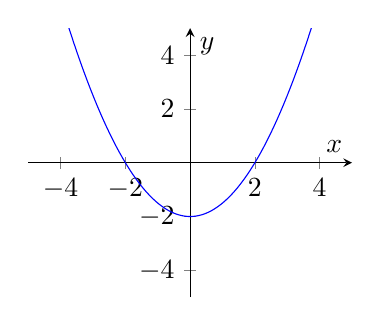
\begin{tikzpicture}
    \begin{axis}[
      scale = .6,
      axis lines = center,
      xlabel = $ x $,
      ylabel = $ y $,
      ymin = -5, ymax = 5,
      xmin = -5, xmax = 5
    ]
      \addplot[domain = -5:5, color = blue, samples = 100] {0.5*x^2 - 2};
    \end{axis}
  \end{tikzpicture}}
\end{center}
This happens in two situations:
\begin{itemize}
  \item $ a $ is positive and $ c - \frac{b^2}{4a} $ is less than zero. Hence $ c < \frac{b^2}{4a} $, $ 4ac < b^2 $, and $ b^2 - 4ac > 0 $.
  \item $ a $ is negative and $ c - \frac{b^2}{4a} $ is greater than zero. Hence $ c > \frac{b^2}{4a} $, $ 4ac < b^2 $, and $ b^2 - 4ac > 0 $.
\end{itemize}

In either case, $ b^2 - 4ac > 0 $.

\subsubsection*{Case II: one $ x$-intercept}
\begin{center}
  \fbox{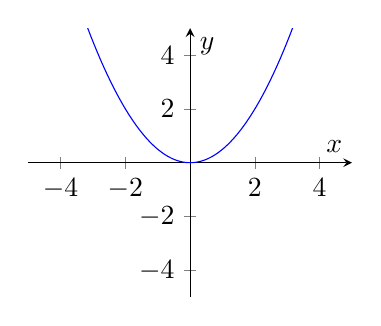
\begin{tikzpicture}
    \begin{axis}[
      scale = .6,
      axis lines = center,
      xlabel = $ x $,
      ylabel = $ y $,
      ymin = -5, ymax = 5,
      xmin = -5, xmax = 5
    ]
      \addplot[domain = -5:5, color = blue, samples = 100] {0.5*x^2};
    \end{axis}
  \end{tikzpicture}}
\end{center}

This happens precisely when the vertex is sitting on the $ x$-axis, so $ c - \frac{b^2}{4a} = 0 $ and $ b^2 - 4ac = 0 $.

\subsubsection*{Case III: no $ x$-intercepts}
\begin{center}
  \fbox{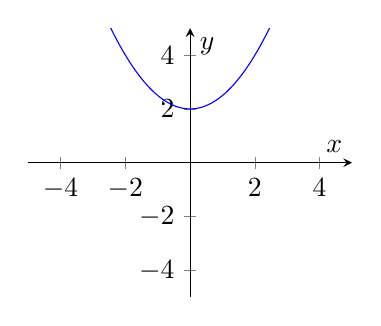
\begin{tikzpicture}
    \begin{axis}[
      scale = .6,
      axis lines = center,
      xlabel = $ x $,
      ylabel = $ y $,
      ymin = -5, ymax = 5,
      xmin = -5, xmax = 5
    ]
      \addplot[domain = -5:5, color = blue, samples = 100] {0.5*x^2 + 2};
    \end{axis}
  \end{tikzpicture}}
\end{center}

This happens in two situations:
\begin{itemize}
  \item $ a $ is positive and $ c - \frac{b^2}{4a} $ is greater than zero. Hence $ c > \frac{b^2}{4a} $, $ 4ac > b^2 $, and $ b^2 - 4ac < 0 $.
  \item $ a $ is negative and $ c - \frac{b^2}{4a} $ is less than zero. Hence $ c < \frac{b^2}{4a} $, $ 4ac > b^2 $, and $ b^2 - 4ac < 0 $.
\end{itemize}

In either case, $ b^2 - 4ac < 0 $.

Notice that the quantity $ b^2 - 4ac $ tells us the nature of the roots in every case; it is known as the \emph{discriminant} of
the quadratic (and I denote it by $ \Delta_2 $). We have therefore proved the following
\begin{thm}
  Suppose $ f(x) = ax^2 + bx + c $. Then:
  \begin{itemize}
    \item If $ b^2 - 4ac < 0 $, then $ f(x) = 0 $ has no solutions.
    \item If $ b^2 - 4ac = 0 $, then $ f(x) = 0 $ has precisely one solution.
    \item If $ b^2 - 4ac > 0 $, then $ f(x) = 0 $ has precisely two solutions.
  \end{itemize}
\end{thm}

If we look at the quadratic equation again,
\begin{displaymath}
  x = \frac{-b \pm \sqrt{b^2 - 4ac}}{2a},
\end{displaymath}
notice that the discriminant appears underneath the square root sign and so it doesn't need to be memorised seperately.

\clearpage
\subsection*{Questions}
\begin{questions}
\fullwidth{\subsubsection*{Solving Quadratics}}
  \question For each quadatic equation,
            \begin{itemize}
              \item rewrite it into vertex form by completing the square if required;
              \item graph the parabola it describes; and
              \item calculate the $ x$-intercept(s) of the parabola, if it has any.
            \end{itemize}
    \begin{parts}
      \part $ y = x^2 + 1 $
      \part $ y = x^2 + x $
      \part $ y = x^2 - 4x + 4 $
      \part $ y = x^2 + 2x + 3 $
      \part $ y = -x^2 + 4x - 2 $
      \part $ y = 2x^2 + 2x + 2 $
    \end{parts}
  \question Show that if $ x^2 - bx + c = 0 $, then $ b $ is the sum of the solutions of the equation.
  \question This question is revision from Level 1.
    \begin{parts}
      \part Justify, with mathematical reasoning, the following statement: the roots of the equation $ (x - \alpha)(x - \beta) = 0 $ are $ \alpha $ and $ \beta $.
      \part Give a quadratic equation with roots $ -1 $ and $ 6 $.
    \end{parts}
  \question Find all the y-intercepts of $ -(x^2 + 2x - 3)(4x^2 - 6x + 2) = y $.
  \question Factorise and solve $ 5x^2 - 9x - 2 = 0 $.
  \question Consider the quadratic equation $ x^2 + bx + c = 0 $.
    \begin{parts}
      \part Calculate $ b $ and $ c $ such that the quadratic equation has solutions $ -1 $ and $ 3 $.
      \part Find the location of the vertex of the corresponding parabola, $ y = x^2 + bx +c $.
    \end{parts}
  \question Solve $ \frac{x^2 + 5x + 2}{x + 2} = 3 $.
  \question Talia used timber to form the exterior sides of her rectangular garden. The length
            of the garden is $ x $ metres, and its area is \SI{50}{\metre\squared}.
    \begin{parts}
      \part Show that the perimeter of the garden is given by $ 2x + \frac{100}{x} $.
      \part If she uses \SI{33}{\metre} of timber to build the sides, find the dimensions of the garden.
    \end{parts}
  \question David and Sione are competing in a cycle race of \SI{150}{\kilo\metre}. Sione cycles on average \SI{4}{\kilo\metre} per hour
            faster than David, and finishes half an hour earlier than David. Find David's average speed. \textit{You MUST use algebra to
            solve this problem. Note that $ \text{average speed} = \frac{\text{distance}}{\text{time}} $.}
  \question Simplify fully $ \dfrac{2x^2 - 8}{x^2 - 2x - 8} $.
  \question The equation $ (x + 2) - 3\sqrt{x + 2} - 4 = 0 $ has only one real solution. Find the value of $ x $.
  \question Check, by direct substitution, that both
            \begin{displaymath}
              x = \frac{-b + \sqrt{b^2 - 4ac}}{2a} \text{ and } x = \frac{-b - \sqrt{b^2 - 4ac}}{2a}
            \end{displaymath}
            are solutions of $ ax^2 + bx + c = 0 $.
  \question
    \begin{parts}
      \part Suppose that it is known that one solution of $ x^2 + bx + c $ is four times the other (i.e. the two solutions are $ \alpha $ and $ 4\alpha $).
            Show that $ c = 4b^2/25 $.
      \part Conversely, show that one solution of $ x^2 + bx + \frac{4b^2}{25} $ is four times the other, no matter the value of $ b $.
      \part Show that one solution of $ 3x^2 + 15x + 12 $ is four times the other.
    \end{parts}
  \question (Challenge problem.) Let $ AB $ be the diameter of a circle centred at $ O $. Draw the circles with diameters $ AO $ and $ OB $; draw a
            third circle centred at $ T $, tangent to all three existing circles. If the radius of the circle at $ T $ is 8,
            what is the length $ d(A,B) $?

  \fullwidth{\subsubsection*{Classifying Roots}}
  \question Without explicitly computing them, how many solutions does each quadratic equation have? Don't use the discriminant
            to decide for all four.
    \begin{parts}
      \part $ 0 = x^2 + 2 $
      \part $ 3 = 3x^2 + 3x $
      \part $ 1 = -x^2 - 2x $
      \part $ 0 = 2x^2 - 12x + 18 $
    \end{parts}
  \question Find $ k $ such that $ x^2 + 3kx - 2 = 0 $ has precisely one solution.
  \question The equation $ (2x - 3)(x + 4) = k $ has only one real solution; find the value of $ k $.
  \question Find all $ t $ such that the parabolae described by $ y = tx^2 + x + 1 $ and $ y = -2x^2 - tx + 1 $ meet at precisely one point.
  \question By considering the quadratic formula, give another proof that the discriminant `encodes' the nature of the roots of the quadratic.
  \question The quadratic equation $ mx^2 - (m + 2)x + 2 = 0 $ has two positive real roots. Find the possible
            value(s) of $ m $, and the roots of the equation.
  \question For what values of $ k $ does the parabola described by
            \begin{displaymath}
              y = x^2 + (3x - 1)x + (2k + 10)
            \end{displaymath}
            never touch the $x$-axis?
  \question Find the possible values of $ d $ if one or more real solutions exist for $ x^2 + 5x - 1 = d(x^2 + 1) $. Interpret
            your answer geometrically.
  \question How many real roots does $ x^3 - 4x^2 + 7x - 4 $ have?
  \question Find expressions in terms of $ m $ and $ n $ for the roots of the equation
            \begin{displaymath}
              \frac{x - m}{x - n} = \frac{2(x + m)}{x + n}.
            \end{displaymath}
            Give an inequality, in terms of $ m $ and $ n $, so that the equation has two distinct roots.
  \question
    \begin{parts}
      \part Two positive numbers have sum 25 and product 136. What are the two numbers?
      \part For which numbers $ S $ and $ P $ is it possible to find at least one pair of real numbers with sum $ S $ and product $ P $?
    \end{parts}
  \question Let $ \alpha $ and $ \beta $ be the roots of $ x^2 + bx + c $.
    \begin{parts}
      \part Show that $ \alpha^2 + \beta^2 = (-b)^2 - 2c $.
      \part Conclude that $ \Delta_2[x^2 + bx + c] = (\alpha - \beta)^2 $.
    \end{parts}
  \question Let $ \rho $ be positive. Suppose $ P $ and $ Q $ are points such that $ \abs{PQ} \leq 2\rho $;
            show that the two circles of radius $ \rho $ with centres $ P $ and $ Q $ intersect;
            show that they intersect in exactly one place if and only if $ \abs{PQ} = 2\rho $.
\end{questions}

\end{document}
